\documentclass[nooutcomes]{ximera}
%% handout
%% space
%% newpage
%% numbers
%% nooutcomes


\newcommand{\RR}{\mathbb R}
\renewcommand{\d}{\,d}
\newcommand{\dd}[2][]{\frac{d #1}{d #2}}
\renewcommand{\l}{\ell}
\newcommand{\ddx}{\frac{d}{dx}}
\newcommand{\dfn}{\textbf}
\newcommand{\eval}[1]{\bigg[ #1 \bigg]}

\usepackage{multicol}

\renewenvironment{freeResponse}{
\ifhandout\setbox0\vbox\bgroup\else
\begin{trivlist}\item[\hskip \labelsep\bfseries Solution:\hspace{2ex}]
\fi}
{\ifhandout\egroup\else
\end{trivlist}
\fi} %% we can turn off input when making a master document
\usepackage{fullpage}

\title{Section 3.1: Introducing the Derivative}  

\begin{document}
\begin{abstract}		\end{abstract}
\maketitle

%problem1
\begin{problem}
 Recall the following two figures depicting the same graph $y=f(x)$ and the same two lines, and the same two points $P$ and $Q$:
  \[
    \begin{array}{lr}
      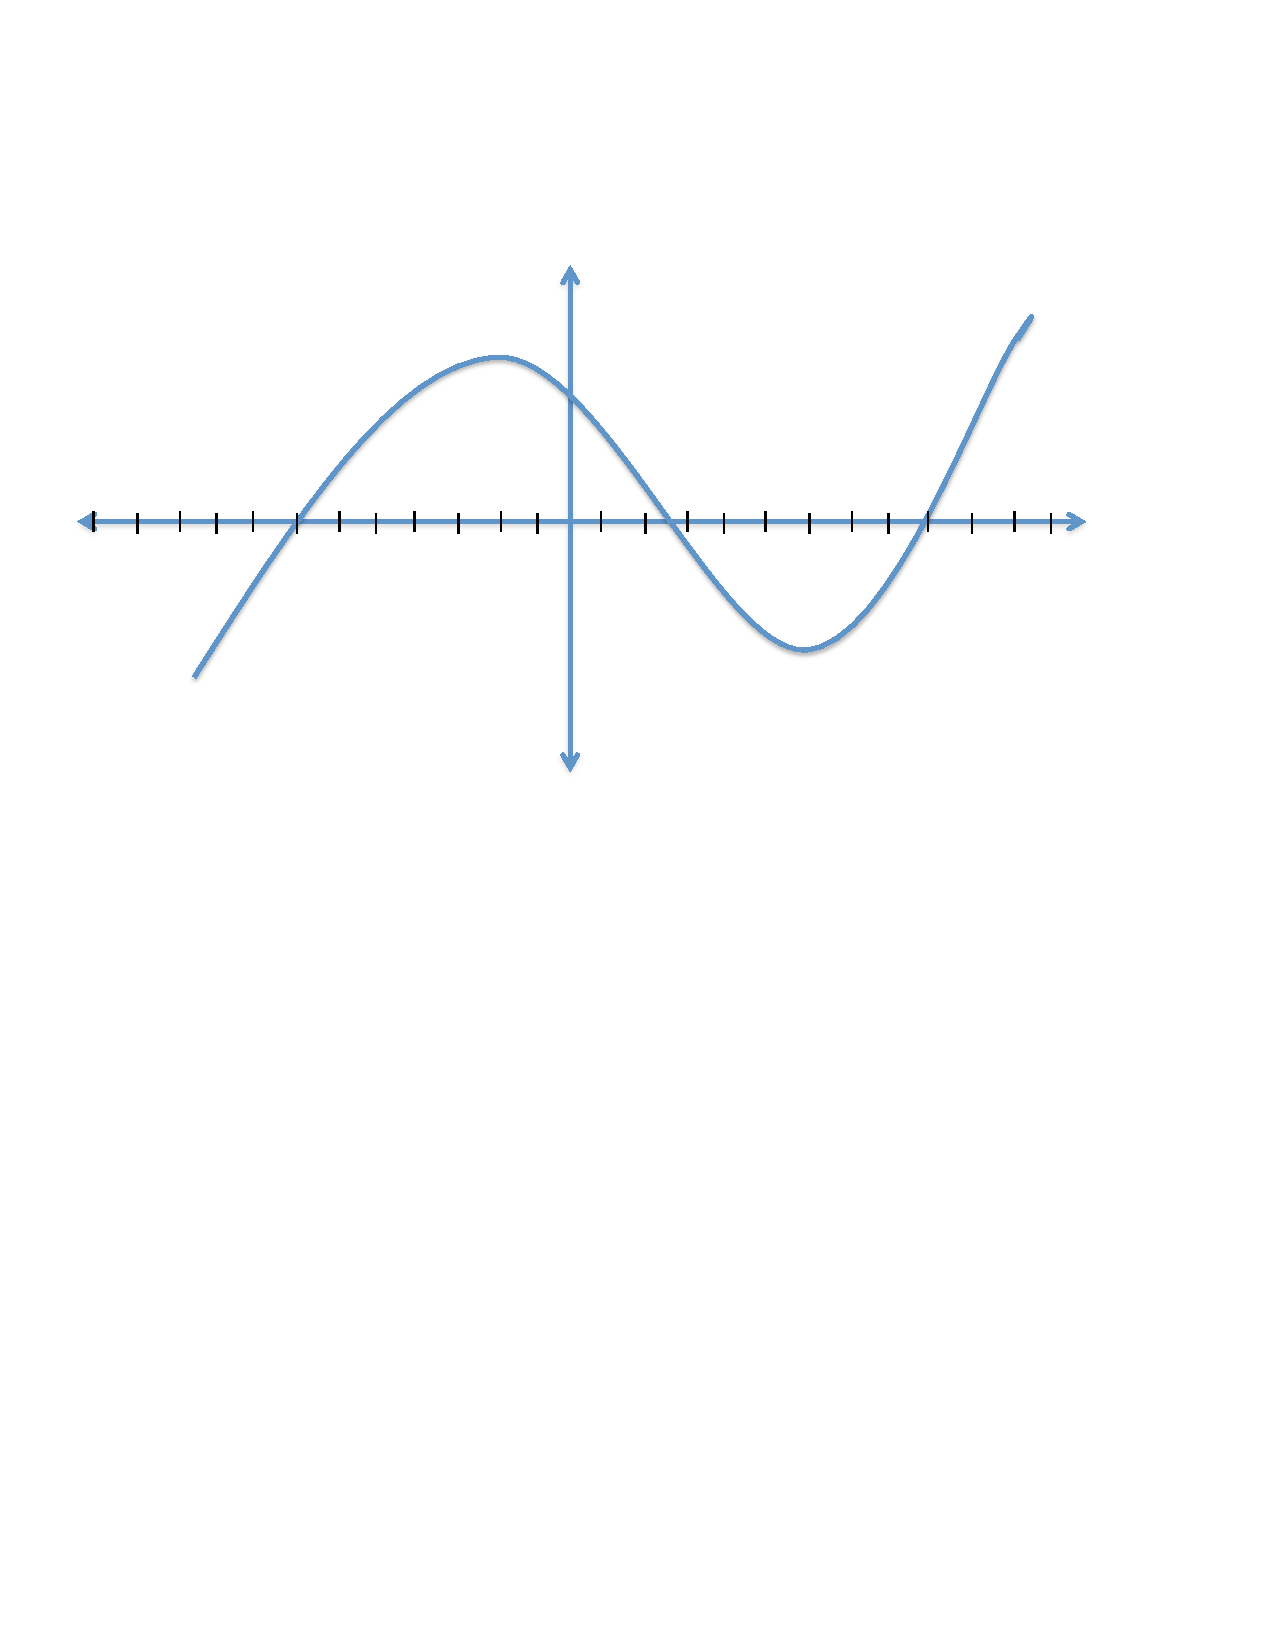
\includegraphics[trim= 150 350 250 180]{Figure2.pdf} &		   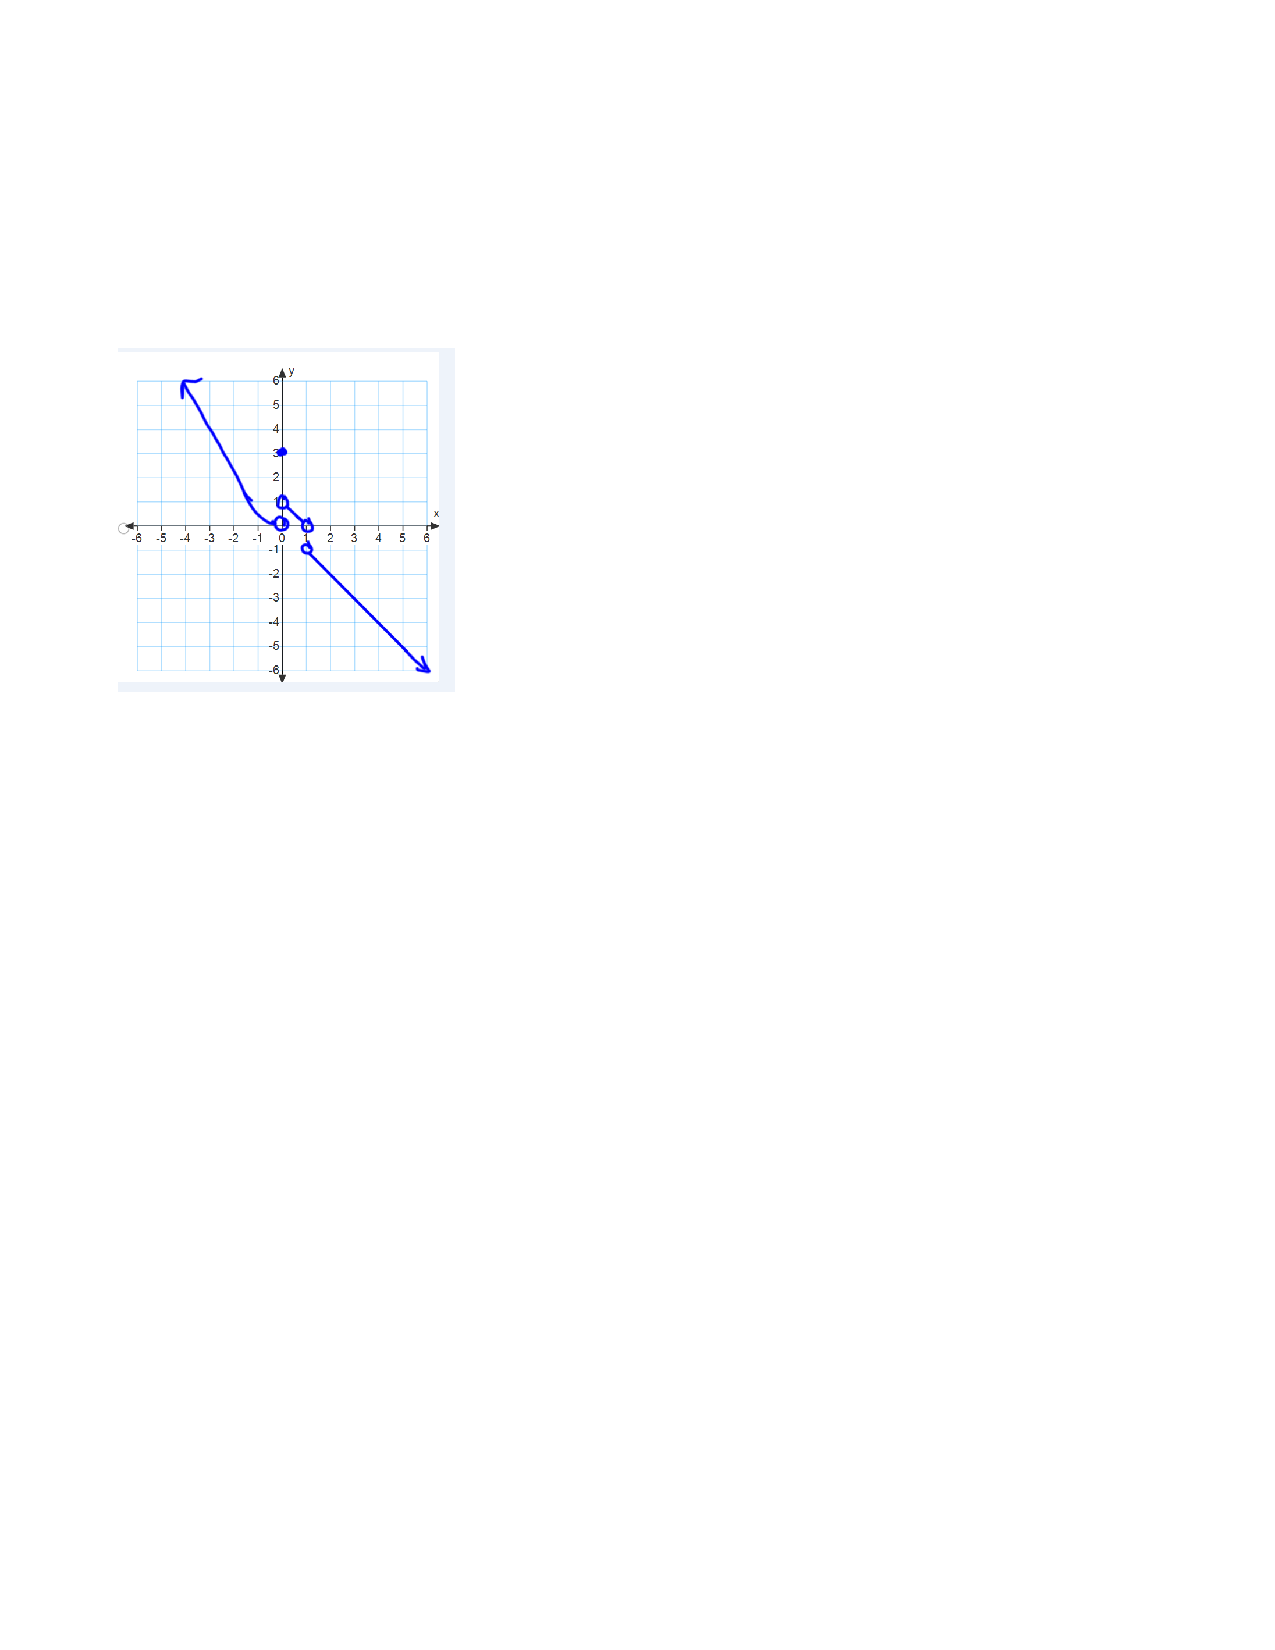
\includegraphics[trim= 140 350 250 180]{Figure3.pdf}
    \end{array}
  \]
  \begin{enumerate}
    \item
      In Figure 1 on the left, what are the coordinates of $P$ and $Q$?  In Figure 2 on the right, what are the coordinates of $P$ and $Q$?

	\begin{freeResponse}
	Figure 1 on the left: $P(a,f(a))$ and $Q(x,f(x))$ \\
	Figure 2 on the right: $P(a,f(a))$ and $Q((a+h),f(a+h))$

	\end{freeResponse}

	\item Express the slope of the secant line through $P$ and $Q$ in terms of the above coordinates for each Figure 1 and Figure 2.

      \begin{freeResponse}
	Figure 1: $\frac{f(x)-f(a)}{x-a}$ 
	Figure 2: $\frac{f(a+h)-f(a)}{h}$
        \end{freeResponse}
	
	\item
	Express the slope of the tangent line at the point $x=P$ in terms of the above coordinates for each Figure 1 and Figure 2.

	\begin{freeResponse}
        	Figure 1:  $ \lim_{x \to a} \frac{f(x)-f(a)}{x-a}$
	Figure 2: $\lim_{h \to 0} \frac{f(a+h)-f(a)}{h}$
      \end{freeResponse}

    \item 
      What is the difference?
      \begin{freeResponse}
	Just the variable we use, $x$ or $h$ where $x=a+h \iff h=x-a$
      \end{freeResponse}


    \item 
      For each of the two graphs, which lines are the secant lines?
      \begin{freeResponse}
        The green line is the secant line in each of the two graphs.        
      \end{freeResponse}

    \item 
      For each of the two graphs, which lines are the tangent lines?
      \begin{freeResponse}
        The red line is the tangent line in each of the two graphs.        
      \end{freeResponse}

  \end{enumerate}
\end{problem}

		
		
%problem2
\begin{problem}
 For each of the following functions find the equation of the tangent line at the given point.
  \begin{enumerate}
    \item
      $f(x) = -5x^2 + 7x - 9$ at $x = 3$.
      \begin{freeResponse}
        Slope of tangent line:
        \begin{align*}
          m_{\mathrm{tan}} = \lim_{x \to 3} \frac{f(x) -f(3)}{x-3}
		&= \lim_{x \to 3} \frac{(-5x^2 + 7x - 9) - (-45 + 21 - 9)}{x-3}  \\
		&= \lim_{x \to 3} \frac{-5x^2 + 7x - 9 + 33}{x-3}  \\
		&= \lim_{x \to 3} \frac{-5x^2 + 7x + 24}{x-3}  \\
		&= \lim_{x \to 3} \frac{(x-3)(-5x -8)}{x-3}  \\
		&= \lim_{x \to 3} (-5x - 8)  \\
		&= -5(3) - 8 = -23.
	\end{align*}
        
        Point on tangent line: $(3, f(3)) = (3, -33)$.

        Equation of tangent line:
        \begin{align*}
          y - f(3) = -23(x-3) &\implies y + 33 = -23x + 69\\
          &\implies y = -23x + 36.
        \end{align*}
      \end{freeResponse}

    \item
      $g(u) = \sqrt{5u-4}$ at $u = 3$.
      \begin{freeResponse}
        Slope of tangent line:
        \begin{align*}
          m_{\mathrm{tan}} = \lim_{h \to 0} \frac{g(3+h) - g(3)}{h}
            &= \lim_{h \to 0} \frac{\sqrt{5(3+h) - 4} - \sqrt{11}}{h}\\
          		&=\lim_{h \to 0} \frac{\sqrt{5(3+h) - 4} - \sqrt{11}}{h} \cdot \frac{\sqrt{5(3+h) - 4} + \sqrt{11}}{\sqrt{5(3+h) - 4} + \sqrt{11}} \\
		&= \lim_{h \to 0} \frac{5(3+h) - 4 - 11}{h \left( \sqrt{5(3+h) - 4} + \sqrt{11} \right) }  \\
		&= \lim_{h \to 0} \frac{5h + 15 - 15}{h \left( \sqrt{5(3+h) - 4} + \sqrt{11} \right) }  \\
		&= \lim_{h \to 0} \frac{5}{\left( \sqrt{5(3+h) - 4} + \sqrt{11} \right) }  \\
		&= \frac{5}{\sqrt{5(3+0) - 4} + \sqrt{11}}  \\
		&= \frac{5}{2 \sqrt{11}}.
        \end{align*}

        Point on tangent line: $(3, g(3)) = (3, \sqrt{11})$.

        Equation of tangent line:
        \begin{align*}
          y - g(3) = \frac{5}{2\sqrt{11}}(u-3)
          &\implies y - \sqrt{11} = \frac{5}{2\sqrt{11}}(u - 3)\\
          &\implies y = \frac{5}{2\sqrt{11}}u - \frac{15}{2\sqrt{11}} + \sqrt{11}.
        \end{align*}
      \end{freeResponse}

    \item
      $\displaystyle s(z) = \frac{z}{z-5}$ at $z = 3$.
      \begin{freeResponse}
        Slope of tangent line:
        \begin{align*}
          m_{\mathrm{tan}}
          &= \lim_{z \to 3} \frac{s(z) - s(3)}{z-3}  \\
		&= \lim_{z \to 3} \frac{\frac{z}{z-5} - \frac{3}{3-5}}{z-3}  \\
		&= \lim_{z \to 3} \frac{\frac{z}{z-5} + \frac{3}{2}}{z-3}  \\
		&= \lim_{z \to 3} \frac{\frac{2z}{2(z-5)} + \frac{3(z-5)}{2(z-5)}}{z-3}  \\
		&= \lim_{z \to 3} \frac{\frac{2z + 3z - 15}{2(z-5)}}{z-3}  \\
		&= \lim_{z \to 3} \frac{5z-15}{2(z-5)} \cdot \frac{1}{z-3}  \\
		&= \lim_{z \to 3} \frac{5(z-3)}{2(z-5)} \cdot \frac{1}{z-3}  \\
		&= \lim_{z \to 3} \frac{5}{2(z-5)}  \\
		&= \frac{5}{2(3-5)} = -\frac{5}{4}.
	\end{align*}

        Point on tangent line: $(3, s(3)) = (3, -3/2)$.

        Equation of tangent line:
        \begin{align*}
          y - s(3) = - \frac{5}{4}(z-3) &\implies y + \frac{3}{2} = - \frac{5}{4}z + \frac{15}{4}\\
          &\implies y = - \frac{5}{4} z + \frac{9}{4}.
        \end{align*}
      \end{freeResponse}
  \end{enumerate}
\end{problem}


%problem3
\begin{problem} Find the equation of the tangent line at the given point.  Then graph the function and its derivative on the same plot.
$f(x)=\sqrt{x+1}$ at $x=3$

	\begin{freeResponse}
	Slope of tangent line:
	\begin{align*}	
	m_{\mathrm{tan}} = \lim_{h \to 0} \frac{f(3+h) - f(3)}{h}&=\lim_{h \to 0}\frac{\sqrt{3+h+1} - \sqrt{4}}{h}\\
	&=\lim_{h \to 0}\frac{\sqrt{4+h} - \sqrt{4}}{h} \cdot \frac{\sqrt{4+h} + \sqrt{4}}{\sqrt{4+h} + \sqrt{4}}\\
	&=\lim_{h \to 0}\frac{4+h-4}{h(\sqrt{4+h} + \sqrt{4})}\\
	&=\lim_{h \to 0}\frac{h}{h(\sqrt{4+h} + 2)}\\
	&=\lim_{h \to 0}\frac{1}{\sqrt{4+h} + 2}\\
	&=\frac{1}{\sqrt{4+0} + 2}\\
	&=\frac{1}{4}
	\end{align*}

        Point on tangent line: $(3, f(3)) = (3, 2)$.

        Equation of tangent line:
        \begin{align*}
          y - f(3) =  \frac{1}{4}(x-3) &\implies y - 2 = \frac{1}{4}x - \frac{3}{4}\\
          &\implies y = \frac{1}{4}x + 1\frac{1}{4}.
        \end{align*}
	        \begin{image}
          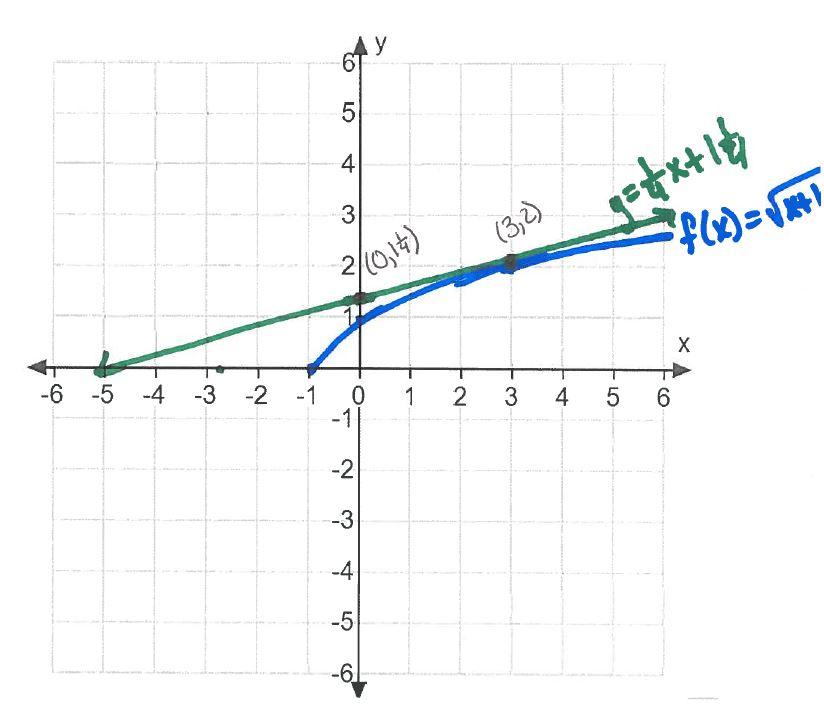
\includegraphics[scale = 0.6]{Figure5.JPG}
        \end{image}

	\end{freeResponse}

\end{problem}

%problem4
\begin{problem}

The graph of a function $p$ and a point in its domain, $b$, are shown in the figure below.
	        \begin{image}
          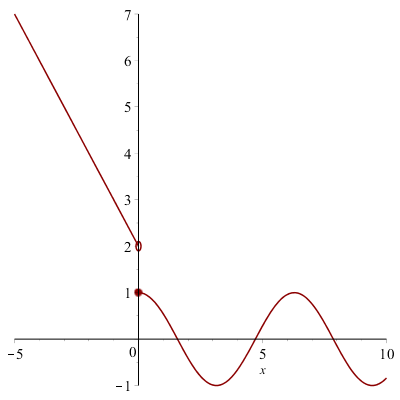
\includegraphics[scale = 0.5]{Figure6.png}
        \end{image}

	\begin{enumerate}
		\item In the figure above, draw and mark clearly the quantity $\Delta y=[p(b)-p(1)]$ and the quantity $\Delta x=b-1$.
		\begin{freeResponse}\hfil
	        \begin{image}
          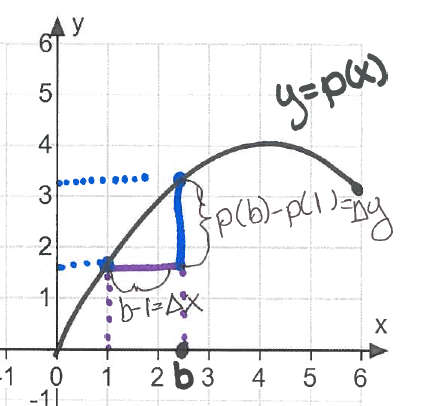
\includegraphics[scale = 0.7]{Figure7.png}
        \end{image}

		\end{freeResponse}

		\item Complete the sentence.  The quotient $\frac{p(b)-p(1)}{b-1}$ is the slope...

		\begin{freeResponse}
			The quotient $\frac{p(b)-p(1)}{b-1}$ is the slope of the secant line through the points $(b,p(b))$ and $(1,p(1))$
		\end{freeResponse}

		\item Complete the sentence.  Provided it exists, the limit $\lim_{x \to 1}\frac{p(x)-p(1)}{x-1}$ is the slope...
		\begin{freeResponse}
			 Provided it exists, the limit $\lim_{x \to 1}\frac{p(x)-p(1)}{x-1}$ is the slope of the tangent line to the curve at the point $(1,p(1))$
		\end{freeResponse}
	\end{enumerate}
\end{problem}



	
%problem5	
\begin{problem} 
The position, $s(t)$, of an object moving along a horizontal line is given by $s(t) = t^2 - 4$.  Where $s$ is in meters and $t$ is in seconds.
\begin{enumerate}
\item
Mark the position of the object on the line at time $t = 1$:
\begin{image}
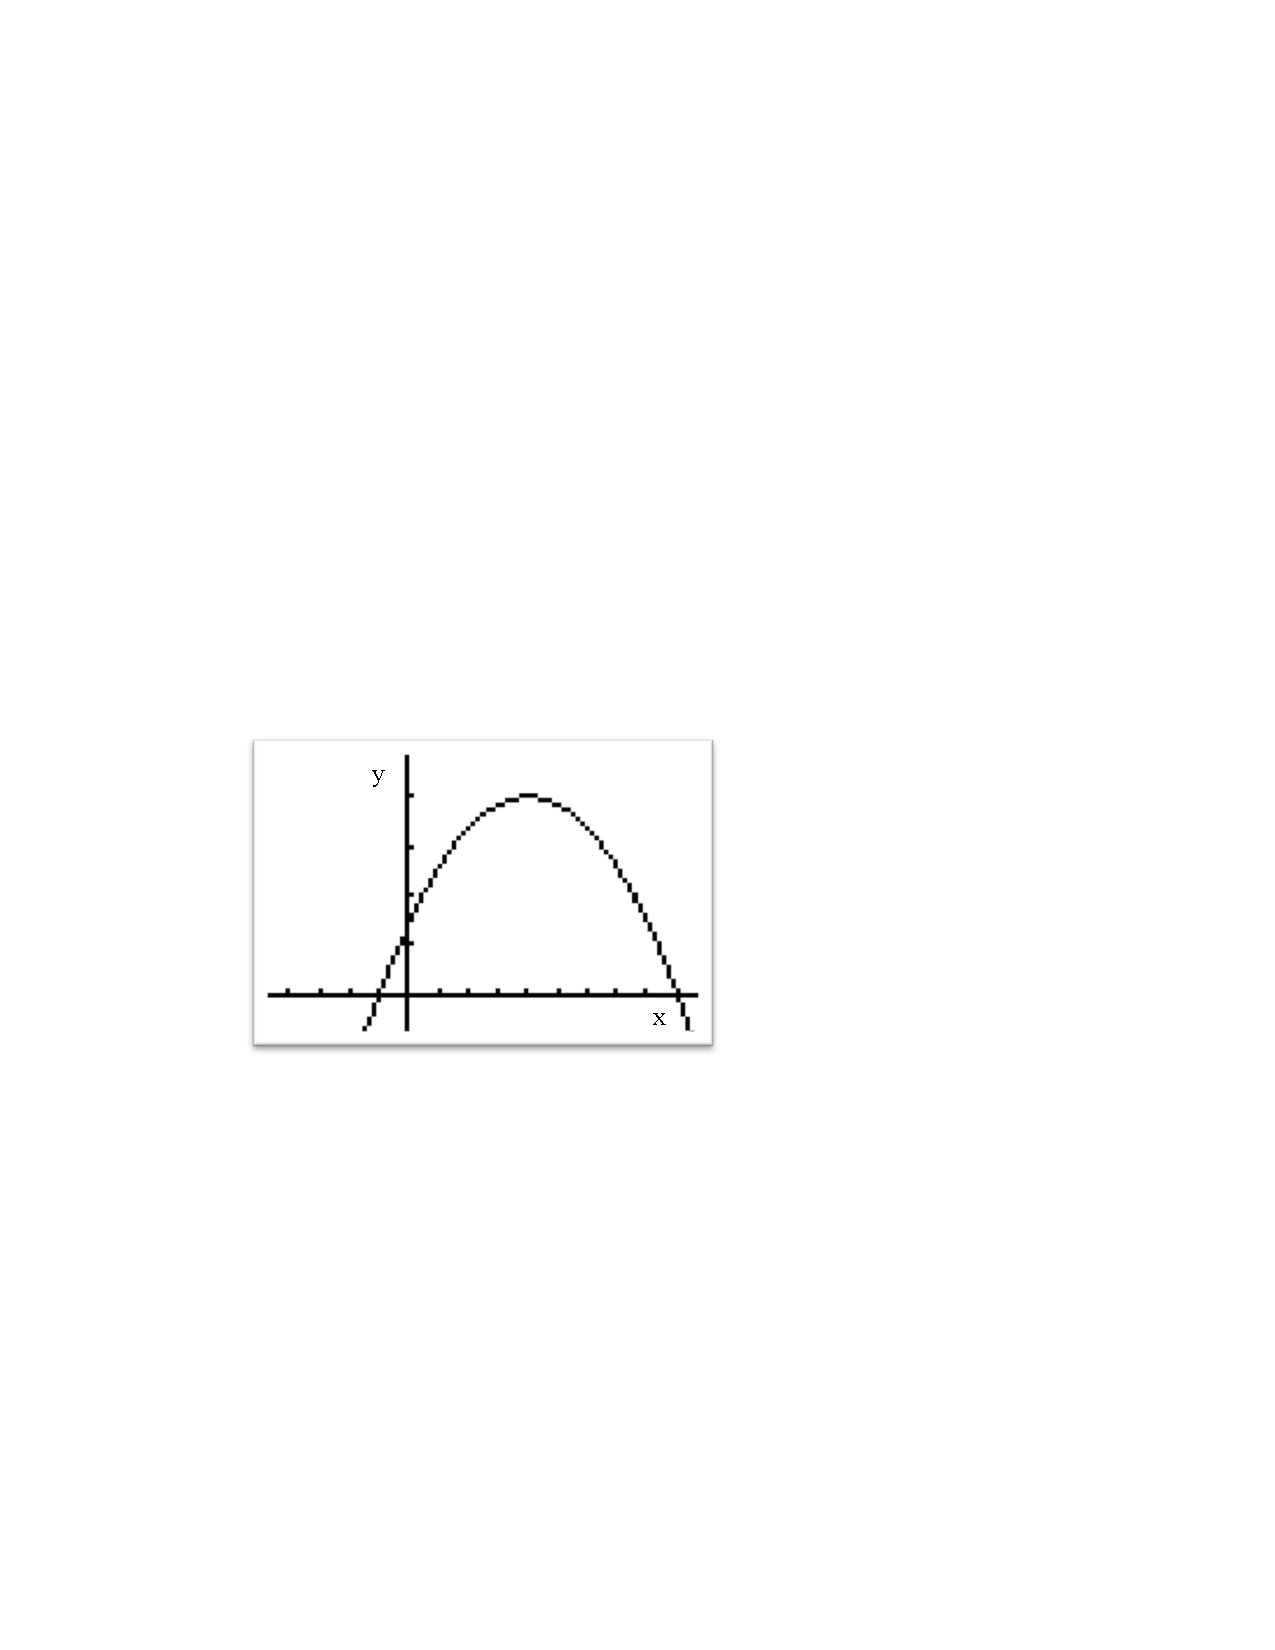
\includegraphics[scale = 1]{Figure9.png}
\end{image} 

\begin{freeResponse}
$s(1)=1^2-4=-3$
\begin{image}
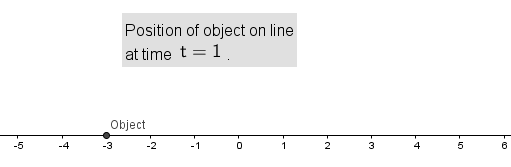
\includegraphics[scale = .8]{Figure8.png}
\end{image}
\end{freeResponse}


\item
Find the average velocity, $v_{\mathrm{AV}}$, of the object during the time interval $[1, 3]$.
\begin{freeResponse}
The average velocity over $[1, 3]$ is
\[
\frac{s(3) - s(1)}{3-1} = \frac{5 - (-3)}{2} = \frac{8}{2} = 4 \text{m/s}
\]
\end{freeResponse}


\item
Compute the average velocity, $v_{\mathrm{AV}}(t)$, of the object during the time interval
\begin{enumerate}
\item
$[1, t]$, for $t > 1$;
\begin{freeResponse}
The average velocity over $[1, t]$ is
\begin{align*}
\frac{s(t) - s(1)}{t-1} &= \frac{(t^2-4) - (-3)}{t-1}\\
&= \frac{t^2-1}{t-1} = t+1.
\end{align*}
\end{freeResponse}

\item
$[t, 1]$, for $0 < t < 1$.
\begin{freeResponse}
The average velocity over $[t, 1]$ is
\begin{align*}
\frac{s(1) - s(t)}{1-t} &=\frac{(-3) - (t^2-4)}{1-t}\\
&= \frac{1-t^2}{1-t} = 1+t.
\end{align*}

Note: $\frac{s(1) - s(t)}{1-t}= \frac{s(t) - s(1)}{t-1}=1+t$
\end{freeResponse}
\end{enumerate}

\item 
Find the instantaneous velocity, $v_{\mathrm{inst}}$, of the object at $t = 1$.
Justify your answer.
\begin{freeResponse}
The instantaneous velocity of the object at $t = 1$ is
\begin{align*}
v_{\mathrm{inst}} &=\lim_{t \to 1}v_{\mathrm{AV}}(t)= \lim_{t \to 1} \frac{s(t) - s(1)}{t-1} \\
&= \lim_{t \to 1} (t+1) = 2.
\end{align*}
\end{freeResponse}


\item
The position-time graph of the function $s$ is given in the figure below.
\begin{image}
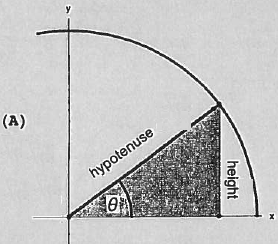
\includegraphics[scale = .7]{Figure10.png}
\end{image}
\begin{enumerate}
\item
Assume $P$ is a point on the graph of $s$.
Fill in the blank.
\[
P = (1, \mbox{\underline{\hspace{2em}}}).
\]
\begin{freeResponse}
$P = (1, \mbox{\underline{$-3$}})$
\end{freeResponse}


\item
Plot the point $P$ and draw the tangent line at this point in the figure above.
\begin{freeResponse} \hfil
\begin{image}
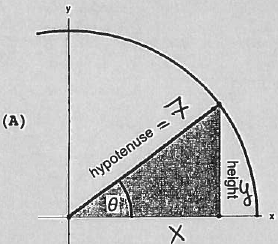
\includegraphics[scale = .7]{Figure11.png}
\end{image}
\end{freeResponse}


\item
Find the slope, $m_{\mathrm{tan}}$, of the tangent line in part (ii).
Explain.
\begin{freeResponse}
The slope of the tangent line at $t = 1$ is the same as the instantaneous velocity at $t = 1$.
Therefore $m_{\mathrm{tan}} = v_{\mathrm{inst}} = 2$.
\end{freeResponse}
\end{enumerate}


\end{enumerate}
\end{problem} 
	
	
	
	
	
	
	

	










								
				
				
	














\end{document} 


















